\documentclass[iop, twocolappendix, numberedappendix, tighten, appendixfloats]{emulateapj}
\citestyle{apj}

\usepackage[stable]{footmisc}
\usepackage{graphicx}
\usepackage{txfonts}
%\usepackage{hyperref}
\usepackage{natbib}
\bibpunct[, ]{(}{)}{;}{a}{}{,}
%\bibliographystyle{./bibtex/apj}

\newcommand{\farc}{\hbox{$.\!\!^{\prime\prime}$}} 
\newcommand{\ergA}{$\rm{erg\,cm^{-2}\,s^{-1}\,\AA^{-1}}$} 
\newcommand{\erg}{$\rm{erg\,cm^{-2}\,s^{-1}}$} 
\newcommand{\kms}{$\rm{km\,s^{-1}}\,$}
\newcommand{\hb}{H$\beta$} 
\newcommand{\ha}{H$\alpha$}
\newcommand{\hg}{H$\gamma$} 
\newcommand{\hi}{\mbox{H\,{\sc i}}} 
\newcommand{\oi}{[\ion{O}{2}]} 
\newcommand{\sii}{[\ion{S}{2}]} 
\newcommand{\oii}{[\ion{O}{2}]} 
\newcommand{\oiii}{[\ion{O}{3}]}
\newcommand{\nii}{[\ion{N}{2}]} 
\newcommand{\hii}{$\rm{H}_2$}
\newcommand{\griz}{$g' r' i' z'$}
\newcommand{\JHK}{$JHK_{\rm{s}}$}
\newcommand{\gK}{$g' r' i' z' JHK_{\rm{s}}$}
\newcommand{\Msun}{$M_\odot$}

\begin{document}
	
	\title{\vspace{-0.5cm}The X-shooter GTO sample of GRB afterglow and host Galaxy spectra}
	\altaffiltext{$^{\dag}$}{Based on observations collected at the European Southern Observatory, Paranal, 
		Chile, Program ID: 084.A-0260, 085.A-009, 086.A-0073, 087.A-0055.}
	
	\author{
		J.~Selsing\altaffilmark{1}, 
		D.~Malesani\altaffilmark{1}, 
		P.~Goldoni\altaffilmark{14}, 
		J.~P.~U. Fynbo\altaffilmark{1}, 
		A.~de~Ugarte~Postigo\altaffilmark{11}, 
		J.~Japelj\altaffilmark{20},
		P.~D'Avanzo,
		Z.~Cano,
		S.~Covino\altaffilmark{10}, 
		V.~D'Elia\altaffilmark{7, 12}, 
		H.~Flores,
		O.~E.~Hartoog\altaffilmark{6},
		J.~Hjorth\altaffilmark{1}, 
		P.~Jakobsson\altaffilmark{5}, 
		T.~Kr\"{u}hler\altaffilmark{1}, 
		A.~Levan,
		A.~Melandri,
		S.~Piranomonte \altaffilmark{7},
		R.~S\'anchez-Ram\'irez\altaffilmark{11},
		S.~Schulze\altaffilmark{17, 18}, 
		N.~R.~Tanvir\altaffilmark{19},
		C.~Th{\"o}ne,
		S.~D.~Vergani\altaffilmark{7, 8},
		P.~M.~Vreeswijk\altaffilmark{3}, 
		D.~J.~Watson\altaffilmark{1},
		K.~Wiersema\altaffilmark{19},
		D.~Xu\altaffilmark{1}
		L.~Christensen\altaffilmark{1},
		A.~De~Cia\altaffilmark{3}, 
		L.~Kaper\altaffilmark{6}, 
		L.~A.~Antonelli,
		F.~Fiore,
		A.~Gomboc,
		P.~Groot,
		F.~Hammer,
		C.~Ledoux\altaffilmark{2}, 
		E.~Maiorano,
		B.~Milvang-Jensen\altaffilmark{1}, 
		E.~Palazzi,
		E.~Pian,
		J.~Schaye,
		G.~Tagliaferri\altaffilmark{7},
		R.~A.~M.~J.~Wijers\altaffilmark{6}
	}
	
	\altaffiltext{1}{Dark Cosmology Centre, Niels Bohr Institute, University of Copenhagen, Juliane Maries Vej 30, 2100 K\o benhavn \O, Denmark}
	\altaffiltext{2}{European Southern Observatory, Alonso de C\'{o}rdova 3107, Vitacura, Casilla 19001, Santiago 19, Chile}
	\altaffiltext{3}{Department of Particle Physics and Astrophysics, Faculty of Physics, Weizmann Institute of Science, Rehovot 76100, Israel}
	\altaffiltext{4}{Th\"uringer Landessternwarte Tautenburg, Sternwarte 5, 07778 Tautenburg, Germany}
	\altaffiltext{5}{Centre for Astrophysics and Cosmology, Science Institute, University of Iceland, Dunhagi 5, IS-107 Reykjavik, Iceland}
	\altaffiltext{6}{Astronomical Institute Anton Pannekoek, University of Amsterdam, Science Park 904, NL-1098 XH Amsterdam, the Netherlands}
	\altaffiltext{7}{INAF-Osservatorio Astronomico di Roma, Via Frascati 33, I-00040 Monteporzio Catone, Italy}
	\altaffiltext{8}{GEPI-Observatoire de Paris, CNRS UMR 8111, Univ. Paris-Diderot, 5 Place Jules Janssen - 92190 Meudon, France}
	\altaffiltext{9}{American River College, Physics and Astronomy Dpt., 4700 College Oak Drive, Sacramento, CA 95841, USA}
	\altaffiltext{10}{INAF, Osservatorio Astronomico di Brera, Via E. Bianchi 46, I-23807 Merate, Italy}
	\altaffiltext{11}{Instituto de Astrof\'{\i}sica de Andaluc\'{\i}a (IAA-CSIC), Glorieta de la Astronom\'{\i}a s/n, 18008, Granada, Spain}
	\altaffiltext{12}{ASI-Science Data Centre, Via Galileo Galilei, I-00044 Frascati, Italy}
	\altaffiltext{13}{Institute of Experimental and Applied Physics, Czech Technical University in Prague, Horska 3a/22, 128 00 Prague 2, Czech Republic}
	\altaffiltext{14}{APC, Astroparticules et Cosmologie, Universite Paris Diderot, CNRS/
		IN2P3, CEA/Irfu, Observatoire de Paris, Sorbonne Paris Cite, 10, Rue Alice Domon et L
		eonie Duquet, 75205 Paris Cedex 13, France}
	\altaffiltext{15}{Max-Planck-Institut f\"{u}r extraterrestrische Physik, Giessenbachs
		tra\ss e, 85748 Garching, Germany}
	\altaffiltext{16}{Universit\`a degli studi di Milano-Bicocca, Piazza della Scienza 3,
		20126, Milano, Italy}
	\altaffiltext{17}{Pontificia Universidad Cat\'{o}lica de Chile, Departamento de Astro
		nom\'{\i}a y Astrof\'{\i}sica, Casilla 306, Santiago 22, Chile}
	\altaffiltext{18}{Millennium Center for Supernova Science}
	\altaffiltext{19}{Department of Physics and Astronomy, University ofLeicester, University Road, Leicester, LE1 7RH, UK}
	\altaffiltext{20}{University of Ljubljana,Department of Physics,Faculty of Mathematics \& Physics,SI}\
	
	\begin{abstract}
		Later
	\end{abstract}
	
	\keywords{Gamma-ray burst: individual: GRB~120815A --- galaxies: high-redshift --- ISM: molecules --- dust, extinction }
	
	\section{Introduction}
	
	\section{Observations}
	
	\LongTables
	
	\begin{deluxetable*}{@{\extracolsep{\fill}}lcccccclc@{}}
		%\tabletypesize{\scriptsize}
		%\rotate
		\tablecaption{The full sample of afterglows or hosts observed in the program.
			We here list the burst names and details of the spectroscopic observations. The
			exposure times and slit widths are given in the order UVB/VIS/NIR. The column
			$\Delta t$ shows the time after trigger when the spectroscopic observation was
			started. Mag$_\mathrm{acq}$ gives the approximate magnitude (typically in the
			$R$-band) of the afterglow in the acquisition image.
			\label{sample}}
		\tablewidth{0pt}
		\tablehead{
			\colhead{GRB} &  \colhead{Exptime} & \colhead{Slit width} & \colhead{Airmass} & \colhead{Seeing} & \colhead{$\Delta t$} & \colhead{Mag$_\mathrm{acq}$} & \colhead{Redshift} & \colhead{Ref}\\
			&  \colhead{(ks)}   & \colhead{(arcsec)} &   & \colhead{(arcsec)} & \colhead{(hr)}       &  & &  \\
		}
		\startdata
		090313$^1$ & 6.9/6.9/6.9     & 1.0/0.9/0.9 & 1.2--1.4  & 1.0  &    45  &  21.6  & 3.3736 & (1) \\
		090530$^1$ & 4.8/4.8/4.8     & 1.0/1.2/1.2 & 1.6--2.2  & 1.5  &    20  &  22    & 1.266 & (2) \\
		090809$^1$ & 7.2/7.2/7.2     & 1.0/0.9/0.9 & 1.2--1.1  & 0.9  &  10.2  &  21    & 2.737  & (2,3) \\
		090926$^1$ & 7.2/7.2/7.2     & 1.0/0.9/0.9 & 1.4--1.5  & 0.9  &    22  &  17.9  & 2.1062 & (4) \\
		091018     & 2.4/2.4/2.4     & 1.0/0.9/0.9 & 2.1--1.8  & 0.8  &   3.5  &  19.1  & 0.9710 & (5) \\  
		091127     & 6.0/6.0/6.0     & 1.0/0.9/0.9 & 1.1--1.2  & 1.0  &   101  &  21.2  & 0.490  & (6) \\
		100205A     & 10.8/10.8/10.8 & 1.0/0.9/0.9 & 1.9--1.8  & 1.0  &    71  &   --   &  --    & (2) \\
		100219A     &  4.8/4.8/4.8   & 1.0/0.9/0.9 & 1.3--1.1  & 0.7  &  12.5  &   23   & 4.667  & (7) \\
		100316B     &  2.4/2.4/2.4   & 1.0/0.9/0.9 & 2.0--2.4  & 0.7  &   0.7  &  18.2  & 1.18   & (2) \\
		100316D-1$^2$ &  7.2/7.2/7.2   & 1.0/0.9/0.9 & 1.2--1.5  & 1.0  &  12  &   --   & 0.059  & (8) \\
		100316D-2   &  2.4/2.4/2.4   & 1.0/0.9/0.9 & 1.2--1.2  & 1.0  &    58  &   --   & 0.059  & (8) \\
		100316D-3   &  2.4/2.4/2.4   & 1.0/0.9/0.9 & 1.2--1.2  & 0.8  &   192  &   --   & 0.059  & (8) \\
		100418A-1   &  4.8/4.8/4.8   & 1.0/0.9/0.9 & 1.6--1.3  & 0.7  &   8.4  &  18.1  & 0.6235 & (9) \\
		100418A-2   &  4.8/4.8/4.8   & 1.0/0.9/0.9 & 1.2--1.3  & 0.6  &    34  &   --   & 0.6235 & (9) \\
		100418A-3   &  4.8/4.8/4.8   & 1.0/0.9/0.9 & 1.2--1.4  & 0.7  &    58  &   --   & 0.6235 & (9) \\
		100424A$^3$ &  4.8/4.8/4.8   & 1.0/0.9/0.9 & 1.1--1.2  & 0.8  &   --   &   --   & 2.465  & (2) \\
		100425A     &  2.4/2.4/2.4   & 1.0/0.9/0.9 & 1.5--1.3  & 0.7  &   4.0  &  20.6  & 1.755  & (2,3) \\
		100621A     &  2.4/2.4/2.4   & 1.0/0.9/0.9 & 1.3--1.4  & 1.0  &   7.1  &   --   & 0.542  & (2) \\
		100625A$^3$ &  4.8/4.8/4.8   & 1.0/0.9/0.9 & 1.1--1.0  & 0.8  &    13  &   --   & 0.452  & (2) \\
		100724A$^4$ &  4.2/4.2/4.2   & 1.0/0.9/0.9 & 1.5--2.3  &      &   0.2  &   --   & 1.288  & (2) \\
		100728B$^5$ &  7.2/7.2/7.2   & 1.0/0.9/0.9 & 1.5--1.1  & 0.5  &    22  &   23   & 2.106  & (2) \\
		100814A-1$^4$ & 0.9/0.9/0.9  & 1.0/0.9/0.9 & 1.9--1.7  & 0.5  &   0.8  &   19   & 1.44   & (2) \\
		100814A-2   &  4.8/4.8/4.8   & 1.0/0.9/0.9 & 1.5--1.2  & 0.6  &   1.4  &   19   & 1.44   & (2) \\
		100814A-3   &  4.8/4.8/4.8   & 1.0/0.9/0.9 & 1.2--1.0  & 0.6  &   99   &   20   & 1.44   & (2) \\
		100816A$^6$ &  4.8/4.8/4.8   & 1.0/0.9/0.9 & 1.8--1.6  & 0.8  &   3.7  &   --   & 0.806  & (2) \\
		100901A     &  2.4/2.4/2.4   & 1.0/0.9/0.9 & 1.5--1.5  & 1.8  &   66   &   --   & 1.408  & (10) \\
		101219A     &  7.2/7.2/7.2   & 1.0/0.9/0.9 & 1.1--1.7  & 2.0  &   3.7  &   --   & 0.718  & (2) \\
		101219B-1   &  4.8/4.8/4.8   & 1.0/0.9/0.9 & 1.6--2.6  & 1.3  &  11.6  &   20   & 0.5519 & (11) \\
		101219B-2   &  7.2/7.2/7.2   & 1.0/0.9/0.9 & 1.2--2.0  & 0.8  &   394  &  22.7  & 0.5519 & (11) \\
		101219B-3   &  7.2/7.2/7.2   & 1.0/0.9/0.9 & 1.4--2.1  & 0.9  &   886  &   --   & 0.5519 & (11) \\
		110128A     &  7.2/7.2/7.2   & 1.0/0.9/0.9 & 2.0--1.6  & 0.9  &   5.5  &  22.5  & 2.339  & (2) \\
		110407A     &  9.6/9.6/9.6   & 1.0/0.9/0.9 & 1.4--1.3  & 2.0  &  12.4  &   23   &  --    & (2) \\
		110709B$^1,3$ &  7.2/7.2/7.2 & 1.0/0.9/0.9 & 1.6--1.1  & 1.0  &   --   &   --   &  --    & (2) \\
		110715A     &  0.6/0.6/0.6   & 1.0/0.9/0.9 & 1.1--1.1  & 1.7  &  12.3  &  18.5  & 0.82  & (2) \\
		%110721A     &  2.4/2.4/2.4   & 1.0/0.9/0.9 & 1.2--1.4  & 2.4  &        &        & 0.382  & (2) \\
		110808A     & 2.4/2.4/2.4    & 1.0/0.9/0.9 & 1.2--1.1  & 1.1  &   3.0  &  21.2  & 1.3488 & (2) \\
		110818A     & 4.8/4.8/4.8    & 1.0/0.9/0.9 & 1.3--1.3  & 1.0  &   6.2  &  22.3  & 3.36   & (2) \\
		111005A$^3$ & 1.2/1.2/1.2    & 1.0/0.9/0.9 & 1.3--1.3  & 0.7  &   --   &  --    & 0.013? & (2) \\
		111008A-1   & 8.8/8.8/8.4    & 1.0/0.9/0.9 & 1.1--1.0  & 1.2  &   8.5  &  21?   & 4.9898 & (12) \\
		111008A-2   & 8.0/8.0/7.2    & 1.0/0.9/0.9 & 1.3--1.0  & 1.0  &  20.1  &  22?   & 4.9898 & (12) \\
		111107A     & 4.8/4.8/4.8    & 1.0/0.9/0.9 & 1.8--1.5  & 0.7  &   5.3  &  21.5  & 2.893  & (2) \\
		111117A$^6$ & 4.8/4.8/4.8    & 1.0/0.9/0.9 & 1.5--1.4  & 0.6  &    38  &  --    & 1.3?   & (2) \\
		111123A-1   & 6.2/6.6/6.6    & 1.0/0.9/0.9 & 1.6--1.1  & 1.0  &  12.2  &  $>$24 & 3.1516 & (2) \\
		111123A-2$^3$ & 2.4/2.4/2.4  & 1.0/0.9/0.9 & 1.0--1.0  & 0.5  &   --   &  --    & 3.1516 & (2) \\
		111129A     & 3.6/3.6/3.6    & 1.0/0.9/0.9 & 1.6--2.1  & 1.7  &        &        &  --    & (2) \\
		111209A-1   & 4.8/4.8/4.8    & 1.0/0.9/0.9 & 1.1--1.2  & 0.8  &  17.7  &  20.1  & 0.677  & (13) \\
		111209A-2   & 9.6/9.6/9.6    & 1.0/0.9/0.9 & 1.2--2.0  & 0.8  &  497   &  23    & 0.677  & (13) \\
		111211A$^1$ & 2.4/2.4/2.4    & 1.0/0.9/0.9 & 1.4--1.6  & 0.6  &   31   &  19.5  & 0.478  & (2) \\
		111228A     & 2.4/2.4/2.4    & 1.0/0.9/0.9 & 1.4--1.4  & 0.9  &  15.9  &  20.1  & 0.716  & (2) \\
		120118B$^3$ & 3.6/3.6/3.6    & 1.0/0.9/0.9 & 1.1--1.0  & 1.0  &   --   &  --    & 2.943  & (2) \\
		120119A-1   & 2.4/2.4/2.4    & 1.0/0.9/0.9 & 1.1--1.1  & 0.6  &   1.4  &   17   & 1.728  & (2) \\
		120119A-2   & 1.2/1.2/1.2    & 1.0/0.9/0.9 & 1.8--1.9  & 0.6  &   4.5  &   20   & 1.728  & (2) \\
		120119A-3$^3$ & 4.8/4.8/4.8  & 1.0/0.9/0.6JH & 1.0--1.1  & 1.1 &   --   &   --   & 1.728  & (2) \\
		120211      &                &             &           &      &        &         & 2.346 & (2) \\
		120224A     & 2.4/2.4/2.4    & 1.0/0.9/0.9 & 1.7--2.1  & 1.4  &  19.8  &   22.3 &  --    & (2) \\
		120311A     & 2.4/2.4/2.4    & 1.0/0.9/0.9 & 1.6--1.4  & 0.6  &   3.7  &   21.6 &  --    & (2) \\
		120327A-1   & 2.4/2.4/2.4    & 1.0/0.9/0.9 & 1.6--1.4  & 0.5  &   2.1  &   18.8 & 2.815  & (14) \\
		120327A-2   & 4.2/4.2/4.2    & 1.0/0.9/0.9 & 1.0--1.1  & 1.0  &    29  &   22.5 & 2.815  & (14) \\
		120404A     & 9.6/9.6/9.6    & 1.0/0.9/0.9JH & 1.7--1.3 & 1.3 &  15.7  &   21.3 & 2.876  & (2) \\
		120422A-1   & 4.8/4.8/4.8    & 1.0/0.9/0.9 & 1.3--1.3  & 0.6  &  17.2  &   22.0 & 0.283  & (15) \\
		120422A-2   & 4.8/4.8/4.8    & 1.0/0.9/0.9 & 1.3--1.4  & 0.9  &  113   &   --   & 0.283  & (15) \\
		120422A-3   & 4.8/4.8/4.8    & 1.0/0.9/0.9 & 1.4--1.7  & 1.0  &  210   &   --   & 0.283  & (15) \\
		120422A-4   & 4.8/4.8/4.8    & 1.0/0.9/0.9JH & 1.3--1.4 & 0.6  & 449   &   --   & 0.283  & (15) \\
		120422A-5   & 4.8/4.8/4.8    & 1.0/0.9/0.9JH & 1.3--1.6 & 0.8  & 593   &   --   & 0.283  & (15) \\
		120422A-6   & 4.8/4.8/4.8    & 1.0/0.9/0.9JH & 1.7--2.4 & 2.5  & 882   &   --   & 0.283  & (15) \\
		120422A-7   & 4.8/4.8/4.8    & 1.0/0.9/0.9JH & 1.5--1.9 & 1.3  & 906   &   --   & 0.283  & (15) \\
		120712A     & 4.8/4.8/4.8    & 1.0/0.9/0.9   & 1.5--2.5 & 1.3  & 10.4  &   21.5 & 4.175  & (2) \\
		120714B     & 4.8/4.8/4.8    & 1.0/0.9/0.9JH & 1.5--1.2 & 1.2  &  7.8  &   22.1 & 0.398  & (2)\\
		120716A$^1$ & 3.6/3.6/3.6    & 1.0/0.9/0.9JH & 1.8--2.6 & 1.0  &  62   &   20.9 & 2.486  & (2) \\
		120722A$^2$ & 4.8/4.8/4.8    & 1.0/0.9/0.9   & 1.3--1.3 & 1.1  & 10.3  &   23.6 & 0.959  & (2) \\
		120805A$^2$ & 3.6/3.6/3.6    & 1.0/0.9/0.9JH & 1.3--1.7 & 0.9  & 218   &   --   & 2.8?   & (2) \\
		120815A     & 2.4/2.4/2.4    & 1.0/0.9/0.9   & 1.3--1.4 & 0.6  &  1.7  &   20   & 2.358  & (16) \\
		120909A     & 1.2/1.2/1.2    & 1.0/0.9/0.9   & 1.6--1.6 & 1.4  &  1.7  &   21   & 3.929  & (2) \\
		120923A     & 9.6/9.6/9.6    & 1.0/0.9/0.9JH & 1.2--1.4 & 1.0  & 18.5  &   --   & $\gtrsim8$ & (2) \\
		121024A     & 2.4/2.4/2.4    & 1.0/0.9/0.9   & 1.2--1.1 & 0.6  &  1.8  &   20   & 2.300  & (17) \\
		121027A     & 8.4/8.4/8.4    & 1.0/0.9/0.9   & 1.3--1.3 & 0.9  &  69   &  21.1  & 1.773  & (2) \\
		121201A     & 4.8/4.8/4.8    & 1.0/0.9/0.9JH & 1.1--1.1 & 0.9  & 12.9  &   23   & 3.385  & (2) \\
		121229A     & 4.8/4.8/4.8    & 1.0/0.9/0.9JH & 1.4--1.2 & 1.4  &  2.0  &  21.5  & 2.707  & (2) \\
		130131B$^3$ & 7.2/7.2/7.2    & 1.0/0.9/0.9JH & 1.3--1.6 & 0.8  &  --   &   --   & 2.539  & (2) \\
		130408A     & 1.2/1.2/1.2    & 1.0/0.9/0.9   & 1.0--1.0 & 1.0  &  1.9  &   20   & 3.758  & (2) \\
		130418A     & 1.2/1.2/1.2    & 1.0/0.9/0.9   & 1.4--1.3 & 1.3  &  4.6  &   18.5 & 1.218  & (2) \\
		130427A     & 1.2/1.2/1.2    & 1.0/0.9/0.9JH & 1.8--1.8 & 0.8  & 16.5  &   19   & 0.340  & (18) \\
		130427B     & 1.2/1.2/1.2    & 1.0/0.9/0.9JH & 1.2--1.0 & 0.8  & 20.3  &   22.7 & 2.78   &  (2) \\
		130603B$^6$ & 2.4/2.4/2.4    & 1.0/0.9/0.9   & 1.4--1.4 & 1.1  &  8.2  &   21.5 & 0.356  & (19) \\
		130606A     & 4.2/4.2/4.2    & 1.0/0.9/0.9JH & 1.7--1.9 & 1.1  &  7.1  &   19   & 5.91   & (20) \\
		130612A     & 1.2/1.2/1.2    & 1.0/0.9/0.9   & 1.3--1.3 & 1.4  &  1.1  &   21.5 & 2.006  & (2) \\
		130615A     & 1.2/1.2/1.2    & 1.0/0.9/0.9   & 2.1--2.2 & 1.0  &  0.8  &   21   & $~3$?  & (2) \\
		130701A     & 1.2/1.2/1.2    & 1.0/0.9/0.9JH & 2.0--2.0 & 1.6  &  5.5  &   19.9 & 1.155  & (2) \\
		\enddata
		\tablenotetext{1}{Not part of the statistical sample}
		\tablenotetext{2}{Spectrum dominated by light from the host galaxy}
		\tablenotetext{3}{Spectrum of the host galaxy taken long after the burst}
		\tablenotetext{4}{RRM observation}
		\tablenotetext{5}{ADC malfunction during observation}
		\tablenotetext{6}{Short burst}
		\tablerefs{
			(1) \citet{Antonio090313}; (2) This work ; (3) Skuladottir (2010);
			(4) \citet{Valerio090926A}; (5) \citet{Klaas091018}; (6) \citet{Vergani091127,Cobb091127}; 
			(7) \citet{christina100219A}; (8) \citet{Buffano} ; (9) de Ugarte Postigo et al. ;
			(10) \citet{Haartog100901A}; (11) \citet{Sparre101219B}; (12) \citet{Sparre111008A};
			(13) \citet{Levanultralong}; (14) D'Elia et al., submitted; (15) \citet{SchulzeSNGRB};
			(16) \citet{Kruehler120815A}; (17} \citet{friis121024A}
	\end{deluxetable*}
	%-------------------------END TABLE---------------------------------------
	
	\section{Results}
	
	\subsection{Spectral resolution}
	The afterglow spectra described in this paper are obtained in Target-of-Opportunity (override) mode.
	In most cases there is therefore little possibility to tweak slit widths to the seeing at the time of observations
	(i.e. to optimise spectral resolution and signal to noise), and almost all our data is therefore taken with a fixed
	set of slit widths and binning, described above. In a fair number of cases, the seeing full width at half maximum (FWHM) 
	is considerably smaller than the silt width, and the delivered spectral resolution will then be determined by the seeing rather 
	than slit width, as afterglows are point sources (this is evidently not the case for extended sources, e.g for host galaxies).
	The delivered resolution for slit width dominated spectra post-reduction and extraction can easily be determined 
	from the bright sky emission lines. For afterglow spectra with very high signal to noise, the delivered spectral resolution 
	can at times be determined from the science data themselves. However, in the presence of multiple velocity components in 
	absorption, other forms of line broadening, and a lack of lines at some redshifts, this is difficult to do at poorer signal to noise ratios
	(the majority of spectra in our sample). A broad starting value for the expect resolution will help fitting of these spectra, and can be important
	in upper limit determination, and for this reason we construct a aim to construct a crude relation between the seeing and the delivered
	resolution at our slit width, binning, and reduction pipeline settings.  
	To this end we use observations of telluric standard stars that are taken with identical instrument settings as our afterglow spectra, usually just after 
	the science data, as part of the ESO X-shooter calibration plan. These spectra have been reduced together with the afterglow spectra, using identical
	pipeline settings with the same version of the pipeline.
	First we fit a Gaussian function in the spatial direction of the trace of the standard star at 792 nm (i.e. in the VIS arm). 
	After this, we fit a series of  20 telluric absorption lines in the telluric standard star spectra with Gaussians, taking care to select transitions 
	that are not almost-resolved multiples, should be intrinsically unresolved, and are in areas with well defined continuum flux.  We pick 34 
	telluric standard stars spanning a range of DIMM seeing values, with the majority between $0.5-1.5 arcsec$. The resulting distribution of 
	spectral FWHM (km/s) as a function of spatial FWHM at 792 nm is fairly well described by a linear relation $a + b*x$, with $x$ the spatial FWHM in pixels (with
	0.15 arc sec per pixel),  $a= 21.4 \pm 1.3$ km/s, $b=1.4 \pm 0.2$. We use this linear relation as a 
	way to estimate the spectral resolution for medium to poor signal to noise afterglow spectra in the VIS arm. To extend this to the UVB and NIR arm, we measured
	a series of lines in NIR arm spectra of a subset of 19 sources used for the VIS arm above, and find that the resulting distribution is consistent with 
	a simple scaling of the VIS arm relation by the ratio of resolutions of the NIR and VIS arm for unresolved, slit filling, sources as given on the ESO instrument website.
	The UVB arm contains no suitable absorption lines to use, and we therefore use a scaled value as in the NIR arm.
	While this simple method is not terribly accurate (for one, the spatial profile of the trace is not a perfect Gaussian), but it gives a sufficiently accurate estimate for the analysis of these poor signal to noise science spectra. 
	
	
%	\begin{figure}
%		%\vspace{11pc}   
%		%\includegraphics[width=10cm]{060218/6273fig1.ps}
%		\centerline{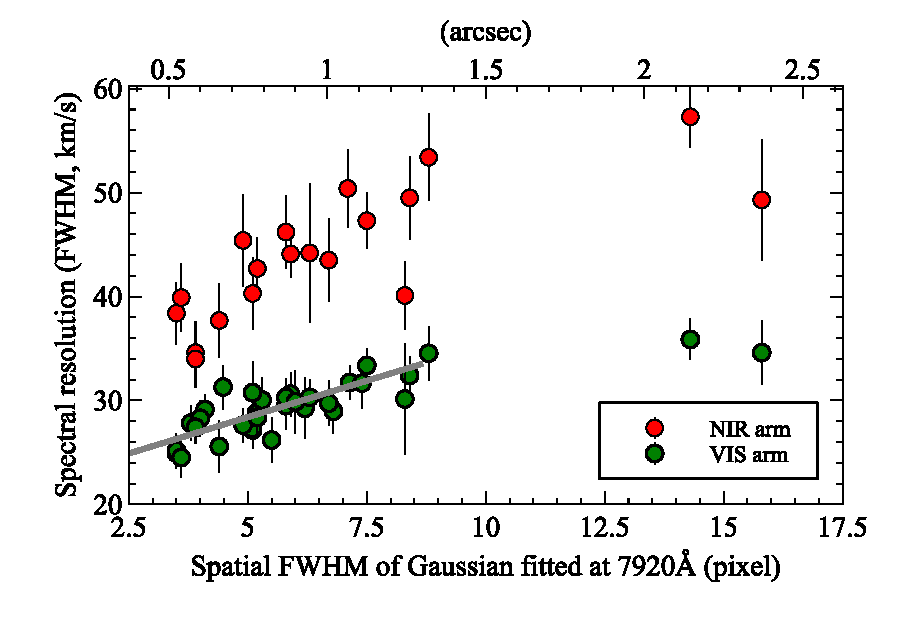
\includegraphics[width=8cm]{Resolution/resolution_paper.eps}}
%		\caption{Green datapoints show the FWHM (km/s) of Gaussian fits to unresolved telluric absorption lines in the VIS spectra, as a function of the FWHM of a Gaussian fit onto the trace in spatial direction at  792 nm. The lower horizontal axis is in units pixels, the top axis in arc seconds. The red datapoints show a subsample of NIR spectra.
%			The grey line shows a linear fit to the VIS datapoints. }
%		\label{fig:res}
%	\end{figure}
	
	\subsection{Correction for offsets in the wavelength calibration}    
	
	X-shooter, being installed at the VLT Cassegrain focusi is  prone to
	flexures during operations. The flexures modify the projection of the slit
	on the detector with respect to the one obtained in daytime calibration. 
	This require a modification of the wavelength solution in order to
	process correctly the night-time data. Part of this correction
	is performed by the pipeline using the frames taken
	during X-shooter Active Flexure Compensation procedure
	\footnote{X-shooter User Manual available at https://www.eso.org/sci/facilities/paranal/instruments/xshooter/doc.html}
	We corrected the remaining part using as a reference the sky
	emission lines present in the observed data.
	
	
	For every afterglow observation we reduced one frame individually in STARE mode without
	sky subtraction obtaining $\sim$ 100 sky spectra. The sky line list compiled at ESO for
	the E-ELT
	study\footnote{http://www.eso.org/sci/facilities/eelt/science/drm/tech\_data/data/optical\_ir\_sky\_lines.dat}
	from the work of (Hanuschik, 2003, A\&A, 407, 1157) and (Rousselot et al. (2000, A\&A, 354, 1134), was used as a reference.
	From this list, we selected a subset of bright and isolated lines. In the case of the OH doublets, unresolved at X-shooter resolution, we took as line position the average between the blue and red components. To find the offsets of the spectra, we fitted gaussians near the
	expected positions under IDL using the MPFIT software (Markwardt, 2009, Astronomical Society of the Pacific Conference Series, Vol. 411, ADASS XVII, ed. D.A. Bohlender, D. Durand, \& P. Dowler, 251) and we compared the result to the tabulated values.
	The resulting offsets, which were smaller than 0.1 \AA~in the UVB and VIS data
	and smaller than 0.5 \AA~in the NIR spectra, were applied to the corresponding spectra.
	
	\subsection{Redshifts}
%	\subsection{Notes on Individual objects}
	
	\section{Discussion}
	
	\begin{acknowledgements}
		JPUF, BMJ and DX acknowledge support from the ERC-StG grant EGGS-278202.  The
		Dark Cosmology Centre is funded by the Danish National Research Foundation.  TK
		acknowledges support by the European Commission under the Marie Curie
		Intra-European Fellowship Programme in FP7.  AdUP acknowledges support by the
		European Commission under the Marie Curie Career Integration Grant programme
		(FP7-PEOPLE-2012-CIG 322307).  This work made use of data supplied by the UK
		{\it Swift} Science Data Centre at the University of Leicester.  Finally, we
		acknowledge expert support from the ESO staff at the Paranal and La Silla
		observatories in obtaining these target of opportunity data.
		
	\end{acknowledgements}
	
	\def\aj{AJ}
	\def\araa{ARA\&A}
	\def\apj{ApJ}
	\def\apjl{ApJL}
	\def\apjs{ApJS}
	\def\apss{Ap\&SS}
	\def\aap{A\&A}
	\def\aapr{A\&A~Rev.}
	\def\aaps{A\&AS}
	\def\mnras{MNRAS}
	\def\nat{Nature}
	\def\pasp{PASP}
	\def\aplett{Astrophys.~Lett.}
	
	\bibliographystyle{apj}
	\bibliography{XSGRB_sample}
	%\bibliography{thebib}
	
	
	\newpage
	\appendix
	\section{Notes on Individual objects}
	
	\subsection{GRB090313}
	
	
	
\end{document}


